\chapter{毫米波蜂窝系统基站天线资源分配与优化研究}

\textbf{本章摘要:} 
Mobile crowdsensing (MCS) is an emerging technology that exploits the enormous sensing power of widely used mobile devices to complete sensing tasks in a cost-efficient manner. Among all outstanding issues of current MCS systems, the concern of lacking privacy protection for the sensing data of participants has drawn increasing attention recently. Various privacy-preserving MCS mechanisms have been proposed for the static scenario where users' privacy protection requirements remain unchanged. In practice, however, users' requirements for privacy protection can be time-varying, which further complicates the design of privacy-preserving MCS. In this article, we first give an overview of multiple promising approaches for privacy-preserving MCS, based on which we make a first attempt to explore the privacy-preserving MCS in a dynamic scenario, which is cast as a Markov Decision Process. Specifically, we develop a reinforcement learning based approach, by which the platform can dynamically adapt its pricing policy catering to the varying privacy-preserving levels of participating users. We further use a case study to evaluate the performance of our proposed approach.

\textbf{关键词:}频谱接入;ICPS安全;分布式算法;博弈论
%\keywords{毫米波通信;Massive MIMO;整数规划}

\section{引言}
Recently, mobile crowdsensing (MCS) has emerged as a popular and effective approach for various sensing tasks (e.g., air quality monitoring, civil noise level measurement, and traffic congestion monitoring \cite{waze, hu2015smartroad, cheng2014aircloud}). In the spirit of crowdsourcing, MCS outsources a collection of sensing tasks to human-carried smart devices equipped with various sensors (e.g., camera, micro-phone, GPS, gyroscope, and accelerometer). Compared with conventional sensor networks, MCS can collect fine-grained information in a more flexible and cost-efficient manner. 

Sensing data contributed by mobile users may contain users' sensitive (private) information, thereby giving rise to privacy concerns when being released to an untrusted party. This becomes a key challenge of designing a MCS system, i.e., how to design efficient incentive mechanisms to stimulate users' participation while preserving user privacy. Traditionally, extensive studies have employed economic approaches to design incentive schemes to attract mobile users' participation, such as auction, game theory, and contract theory \cite{jin2016, zhang2016privacy, wang2016value}. One common assumption made in these works is that system parameters such as sensing utility and mobile users' profiles do not change with time. 

Recently, unified crowdsensing platform design has drawn much attention. In such a platform, participated users can simultaneously fulfill multiple complex sensing tasks for different applications, possibly across a long time period. It is possible that users have different privacy protection requirements when completing different sensing tasks. For example, a user may have higher privacy-preserving level when performing a sensing task for medical applications, in contrast to a lower privacy-preserving level for location based applications. Further, their privacy-preserving levels may change over time (e.g., people may raise the privacy-preserving levels for medical applications when they get sick). This calls for a new approach for such dynamic scenarios where the system parameters are time-varying. 

In this article, we first present an overview of existing incentive mechanisms for MCS that designed to meet static privacy protection requirements. We then focus on the dynamic scenario where each participated user is empowered to locally perturb her sensing data according to a self-specified and time-variant privacy-preserving level. Without knowing users' payoff functions and the changing dynamics of their privacy-preserving levels, it is challenging for the platform to determine the pricing policy via offline approaches. To this end, we propose a learning based approach to adaptively adjust the pricing for sensing tasks while preserving mobile users' privacy. Specifically, the MCS system is modeled as a Markov Decision Process, where each state corresponds to the current privacy-preserving levels of all users. Based on the the observed system state and the perceived reward, the platform adapts its pricing policy dynamically to optimize its utility using a Q-learning based algorithm\cite{Sutton98a}. Intuitively, more payment would be awarded to users with low privacy-preserving levels in order to encourage the contribution of high-quality data. Notably, compared with existing solutions, our proposed learning based pricing mechanism does not require any knowledge about mobile users' payoff function, and enables users to autonomously specify their privacy-preserving requirements under different situations. 

The remainder of this article is organized as follows: In Section \ref{sec:s2}, we review a data privacy attack model as well as two effective data perturbation methods. In Section \ref{sec:s3}, we provide an overview of the existing designs that have integrated the data privacy protection with incentive mechanism. Next, in Section \ref{sec:s4}, we study the MCS scenario where users' privacy-preserving requirements are time-varying and propose a Q-learning based dynamic pricing mechanism. Finally, Section \ref{sec:s5} concludes this article.

\section{研究现状Data Privacy in MCS}\label{sec:s2}
In this article, we consider a semi-trustworthy platform, who collects the sensing data provided by the mobile users. In the following, we first introduce the Bayesian attack model that aims to infer users' sensitive sensing data. Then, we introduce the differential privacy mechanism that can effectively combat the Bayesian privacy attack in MCS.

\subsection{Bayesian Privacy Attack Model}
We assume that a mobile user has private sensing data $x\in\ca{X}$ with $\ca{X}$ denoting the domain of the data value. We also assume that an adversary has the \emph{prior} knowledge about the probabilistic distribution $\pi(x)$ of a participated user's sensing result $x\in\ca{X}$, as well as the probability $p(x^*|x)$ under which a sensing data $x\in\ca{X}$ is obfuscated to $x^*\in\ca{X}$. Then, with the observation of $x^*$, the attacker can derive a \emph{posterior} distribution of user's true sensing result, $p(x|x^*)$, based on Bayes' rule\cite{Leye}:
\begin{equation}
p(x|x^*)=\frac{p(x^*|x)\cdot\pi(x)}{\sum_{x'\in\ca{X}}p(x^*|x')\cdot\pi(x')}.
\end{equation}
In order to combat this Bayesian privacy attack, we design a privacy-preserving mechanism that can bound the improvement of the attacker's \emph{posterior} knowledge over her \emph{prior} knowledge. In other words, it is desirable to have the value of $p(x^*|x)$ and $p(x^*|x')$ close enough so that, given the observation $x^*$, the attacker can hardly distinguish $x$ and $x'$. To this end, we resort to the celebrated notion of differential privacy.

\subsection{Data Differential Privacy}
Following \cite{wang2016value}, we define the differential privacy-preserving level of a user as follows.

\begin{df}[Differential-Privacy-Preserving Level]\label{def1}
The differential privacy-preserving level (DPL) of a user, denoted by $\epsilon$, is defined as
\begin{equation}
\epsilon = \max\left\{\ln\left(\frac{p(x^*|x)}{p(x^*|x')}\right)\right\}, ~\forall x, x'\in\ca{X}.
\end{equation}
\end{df}
A user's $DPL$ quantifies the potential leakage of privacy under the \emph{prior} knowledge of attacker by measuring the indistinguishability between the conditional probability of the reported data. It can be easily proved that with $DPL=\epsilon$, the knowledge gain of an attacker, $g=p(x|x^*)/p(x)$, is bounded as $1/e^\epsilon\leq g\leq e^\epsilon$ with \emph{prior} knowledge $p(x)$. Clearly, the smaller the $\epsilon$, the harder for the attacker to correctly infer out the true data, and hence the better the privacy-preserving performance. We next review two local data perturbation methods, by which a certain differential privacy-preserving level for a user's data can be achieved.

\textbf{Laplace mechanism.}
Laplace mechanism is a widely used technique that provides differential privacy gurantees\cite{dwork2014algorithmic}. In this paper, we are interested especially in a variant version of Laplace mechanism, in which a Laplacian noise $\eta\sim Lap(\Delta/\epsilon)$ is added locally to each individual user's data where $\Delta \triangleq \max_{x,x'\in\ca{X}}|x-x'|$ is defined as the local sensitivity and $\epsilon$ is the $DPL$ of that user.  

\textbf{Randomized response.}
Randomized response is another tool that can provide local differential privacy guarantees\cite{dwork2014algorithmic}. With certain probability, the individual user sends a random instance of her real data to the untrusted data collector. The parameters of randomized response mechanism are carefully chosen to limit the platform's ability to learn with confidence about the true value of the data. %As an illustrating example, when the data is one bit binary data, the data owner can flip a biased coin, and report the truth to the platform if the coin comes up head, and tell the opposite answer if it comes up tail. The data owner thus preserves the data privacy due to the coin randomness.

\section{Noise Injection based Privacy-preserving Approaches in MCS}\label{sec:s3}
In this section, we give an overview of several state-of-art privacy-preserving MCS designs that integrate differential-private noise injection with incentive mechanism design. We classify these works according to the types of incentive mechanisms they used, which includes \emph{auction} based approach, \emph{game theory} based approach, and \emph{contract theory} based approach.



\subsection{Auction based Approach}
The (reverse) auction mechanism is one of the most popular approaches for platform-centric MCS incentive mechanism design. In specific, the platform acts as the auctioneer and the mobile users report their bids reflecting their participation costs to the platform. The platform selects the participants and determines the corresponding payments, aiming to minimize the total payment or to maximize the platform utility under the budget constraint, or to maximize the participants' social welfare\cite{DejunJ}. 

In the seminar work by Ghosh and Roth \cite{ghosh2015selling}, an auction mechanism was proposed, where the private data is treated as goods procured by a data analyzer running a survey. Each individual's privacy cost is modeled as a linear function of her differential-privacy-preserving level $\epsilon$. The designed auction mechanism satisfies two fundamental requirements for incentive mechanism design, i.e., truthfulness and individual rationality:
\begin{itemize}
\item Truthfulness: A participated user cannot benefit from bidding untruthfully.
\item Individual Rationality: Each participated user receives a payment that is larger than or equal to her privacy cost.
\end{itemize}
This work\cite{ghosh2015selling} characterizes the tradeoff between the total payment and the result accuracy from the following two perspectives: 1) to minimize the total payment given an accuracy requirement, or 2) to maximize the result accuracy under a payment budget. 

Along this line, Jin \textsl{et al.} developed a combinatorial auction based framework for preserving data privacy in MCS \cite{jin2016}. Specifically, the privacy cost is modeled as part of each user's sensing cost. In addition, the reliability of mobile users, which influences the accuracy of aggregated sensing results, is further considered during the user selection. Related works \cite{zhang2016privacy} considered a setting where the mobile users are embedded in a social network. Worth noting is that both assumed a trusted data collector in their models.

% In addition, they also considered the case of real-time data aggregation in which their proposed mechanism provides long-term incentives aiming to maintain continuous participation. 
%Although the above mentioned works posses some differences in the models they used, all of them apply the Laplacian mechanism for data perturbation. 

\subsection{Game Theory based Approach}
The game theoretic model is another popular approach for incentive mechanism design \cite{DejunJ, he2017exchange,Yang17}. 
%As a user-centric approach, game theory based approach enables mobile users more involvements into the payment determination process. 
Similar to the auction based mechanism design, game-theoretic approaches need to specify a payment policy that incentives users' participation. However, in game based approaches, the participated users are not selected by the platform; instead, given the payment policy of the platform, users make strategic participation decisions. 

Wang \textsl{et al.} in \cite{wang2016value} devised a game-theoretic mechanism in a setting where a data collector purchases users' private data which represents their knowledge about an underlying system state. Different from \cite{ghosh2015selling,jin2016,zhang2016privacy} where a trusted platform carries out centralized data perturbation over aggregated data, an underlying assumption in \cite{wang2016value} is that the data collector is not trustworthy, in which case each participated user is allowed to locally perturb her raw data strategically before releasing it to the data collector. In their game theoretic model, individual users are the players of the game whose actions correspond to their data perturbation strategies. And the pricing strategy is carefully designed by the data collector, so that a Nash equilibrium of the game can be achieved with participated users' privacy cost being compensated and the accuracy requirement of the collected data being satisfied.

\subsection{Contract based Approach}
In a contract-based mechanism, the contract designer would sophistically design a menu of effort-payment pairs to incentivize the participation of individuals with different types, while at the same time optimize its own payoff. Instead of requiring real-time bid information, contract-based approach exploits the statistical information of individuals' costs to determine payment contracts, which overcomes the information asymmetry and reduces communication and computation overhead. In \cite{Kun1}, a contract-based privacy-preserving MCS framework was proposed. Specifically, the platform designs and broadcasts a menu of contracts, each of which specifies one type of differential-privacy-preserving level and the corresponding payment that a user will receive if she agrees with that contract. Each user then chooses one of the contracts that maximizes her utility. The authors derived the quantitative relationship between individual privacy and aggregation accuracy with proper metrics. 

The three approaches reviewed above are summarized in Table 1. Although they applied different mechanism design approaches, their is one common thread: the $DPL$ of each individual user remains unchanged throughout the crowdsensing procedure. In the next section, we extend the current scenario to a more general one, in which case the mobile users' $DPL$s are not static and the platform needs to dynamically adjust the pricing policy to optiize the operation of the MCS system.

\begin{table*}[!htp]
	\caption{Summary of existing data privacy-preserving approaches for mobile crowdsensing}
	\centering
	\tabcolsep=10pt
	\begin{tabular}[c]{|c|c|c|c|c|c|c|c|}
		\hline \label{table:comparison}
		Reference & Mechanism Type & Platform Trusted &  Data Perturbation & $DPL$ & Features \\ \hline\hline
		
		\cite{jin2016}	  & Auction  	   &        Yes		  &	Laplace mechanism	&  Static & Consider users' reliability	\\ \hline

%		\cite{Kun1}	  & Auction	       &        No  	  & Laplace mechanism & Provide long-term incentive mechanism 	\\ \hline
		
		\cite{zhang2016privacy}	  & Auction		   &        Yes 	      & Laplace mechanism  &  Static & Consider social relationship among users	\\ \hline

		\cite{wang2016value}	  & Game		   &        No 	      &   Randomized response	& Static & Analyze users' equilibrium behaviors	\\ \hline

		\cite{Kun1}	  & Contract	   &		No		  & Laplace mechanism & Static & Overcome information asymmetry \\ \hline

		This paper & -- &		No		  & Laplace mechanism  & Dynamic & Apply learning based online pricing	\\ \hline
	\end{tabular}
\end{table*}

\section{Learning based Dynamic Pricing for Privacy-preserving MCS}\label{sec:s4}
In this section, we develop a reinforcement learning approach for the dynamic pricing problem in a MCS system. In the game-based privacy-preserving MCS approach, the computation of the Nash Equilibrium requires the knowledge about the users' payoff functions and $DPL$s, which is challenging to attain. For the contract based approach, the platform needs at least the statistical information of users' privacy cost for the contract design, which may not be available. In the platform-centric auction based approach, users have little power on deciding their participation status. The learning based approach proposed here can be leveraged to address the information asymmetry problem between the platform and mobile users. In addition, it can be applied in the scenario where users' $DPL$s are time-varying.

\subsection{Problem Statement}
We consider a MCS consisting of a semi-trustworthy platform and a set $\ca{N}\triangleq\{1,2,\cdots,N\}$ of $N$ mobile users. We assume the users are confront with Bayesian data inference attack as introduced in Section \ref{sec:s2}, and have varying differential-privacy-preserving levels ($DPL$s). We let $\bot$ denote the choice of not participating into sensing task and let discrete set $E=\{\epsilon_{(1)},\cdots,\epsilon_{(L)}\}$ be the set of possible values of participated users' $DPL$s, with $\epsilon_{(L)}>\cdots>\epsilon_{(1)}>0$. We use $\epsilon_i^t$ to denote the decision made by mobile user $i$ at stage $t\in \{0,1,2,\cdots\}$. In practice, each user $i$ first decides whether to participate or not. Each participated user would specify a semantic privacy preference level among a list of available options such as \emph{low}, \emph{medium}, \emph{high}, or \emph{very high}; and each one of these options corresponds to a value of $DPL$ provided in set $E$. According to Definition \ref{def1}, the smaller the $\epsilon_i^t$, the higher the privacy-preserving level. 

We assume that each user $i$ owns private sensing data, denoted as $x_i\in\cal{X}$, but only reveals a locally perturbed data, denoted as $\tilde{x}_i\in\ca{X}$, to the semi-trusted platform. The vector $\mathbf{d}=[\tilde{x}_1,\cdots,\tilde{x}_S]$ represents all the data collected by the platform, and $r=f(\mathbf{d})$ is the obtained aggregated result via real-valued function $f$. The local data perturbation and data aggregation processes are illustrated in Fig. \ref{pert}.
\begin{figure}[t]
%\hspace{-0.35cm}
\centering
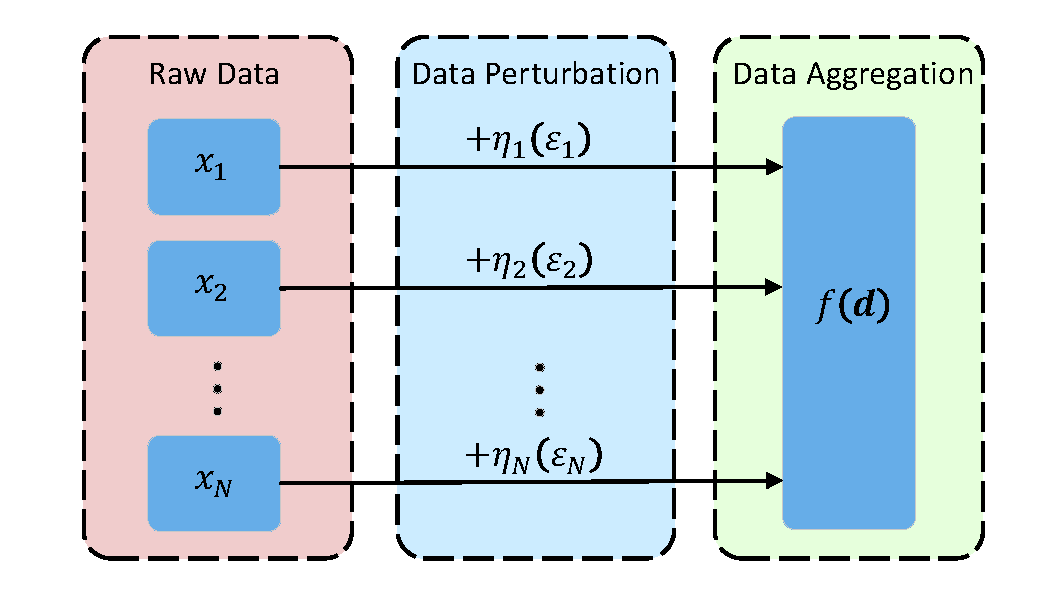
\includegraphics[scale=0.5]{./pic/pert.pdf}
\caption{An illustration of the local data perturbation and data aggregation processes.}\label{pert}
\end{figure}

We define $n_l^t=\sum_{i=1}^N\mathds{1}\{\epsilon^t_i=\epsilon_{(l)}\},~l\in\{1,\cdots,L\}$ as the number of users whose privacy-preserving levels equal to $\epsilon_{(l)}$ at stage $t$, and define the vector $\mathbf{n}^t=(n^t_1,\cdots,n^t_L)$ as the overall privacy-preserving level profile of the mobile crowds. We further denote $\mathbf{p}^t=(p^t_1,\cdots,p^t_L)\in P$ as a pricing profile specified by the platform, where each element $p^t_l\geq0$ indicates the payment to the user with $DPL=\epsilon_{(l)}$. We let $R(\mathbf{n}^t)$ denote the reward perceived by the platform at stage $t$, which is a function of the overall privacy-preserving level profile $\mathbf{n}^t$. The utility of the platform at stage $t$ is defined as the difference between the reward and the total payment, i.e., $u^t_0=R(\mathbf{n}^t)-\mathbf{p}^t\cdot\mathbf{n}^t$. Finally, we define the individual payoff of each user $i\in\ca{N}$ as $u^t_i=p_l^t-\epsilon_{(l)}c^t_i$, where $c^t_i$ is the unit privacy cost of user $i$ at stage $t$. 

\subsection{Q-learning based Dynamic Pricing}
At each stage of our MCS, user $i$ would drop out from participation if the monetary payment could not compensate their privacy loss, i.e., $\max_{\epsilon\in E} u^t_i(\epsilon,\mathbf{p}^t)<0$. Otherwise, user $i$ participates and chooses the $DPL$ that maximizes her payoff, that is, $\epsilon_i^*=\arg\max_{\epsilon\in E}u_i^t(\epsilon,\mathbf{p}^t)$. Next, user $i$ reports to the platform about her $DPL$ as well as the noisy sensing data, which is perturbed in a differentially-private manner parameterized by her $DPL$. Worth noting is that although the platform knows the $DPL$ of each user, she is incapable to restore the original data of each user with high confidence, which fulfills the effective protection of users' data privacy. 
%with probability $1-\delta_i$, and sets her $DPL$ randomly to each of the rest $L-1$ levels with probability $\frac{\delta_i}{L-1}$. The reason of introducing randomness to the decision making is because in reality it might be difficult for the user to perfectly evaluate her payoff

Observing that mobile users' unit privacy costs $\{c^t_i\}_{i\in\ca{N}}$ are time-varying and unknown to the platform and other mobile users, we resort to a learning based approach which is designed to enable the platform to learn out the optimal pricing policy via trial and error. 
\begin{figure}[h]
%\hspace{-0.35cm}
\centering
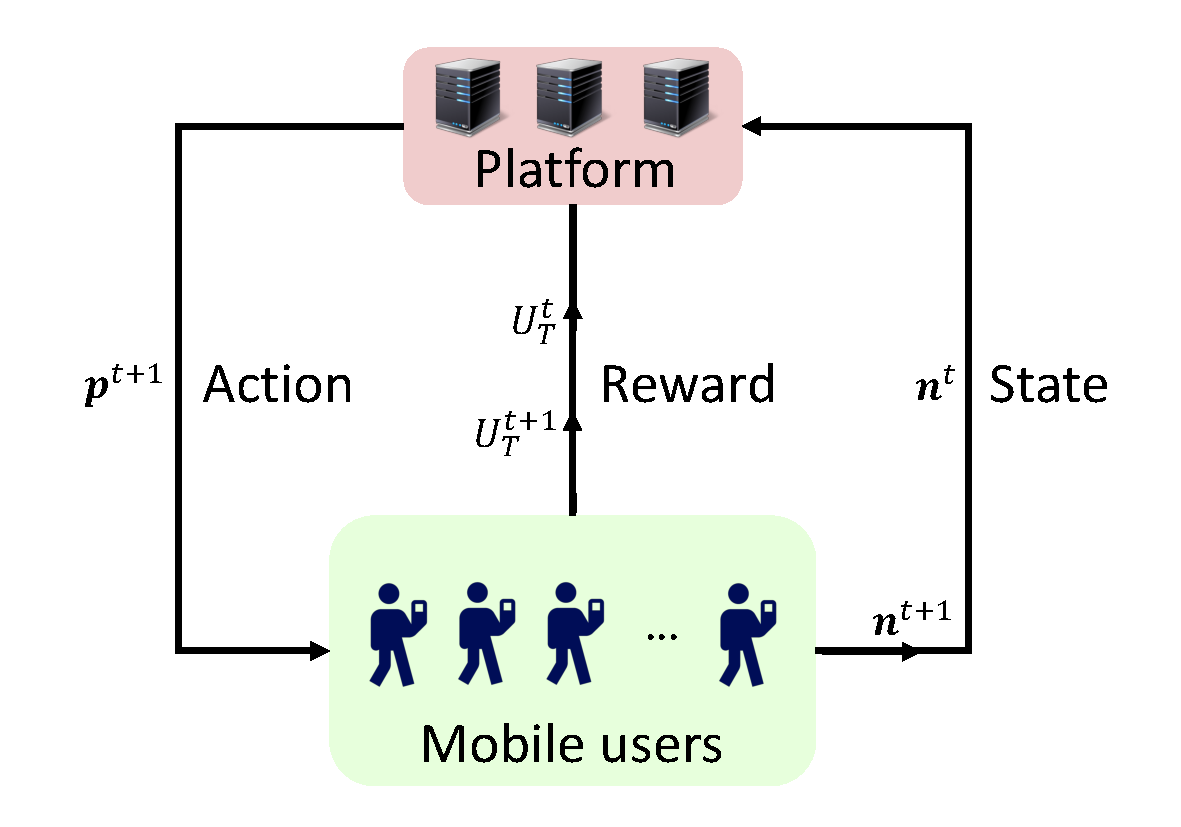
\includegraphics[scale=0.44]{./pic/rl2.pdf}
\caption{An illustration of the principle of the Q-learning based dynamic pricing mechanism.}\label{RL}
\end{figure}
Recently, Xiao \textsl{et al.} casted the interaction between MCS platform and selfish mobile users as a dynamic game and modeled the pricing process of the platform to a Markov Decision Process \cite{Xiao}. Inspired by \cite{Xiao}, we model the MCS platform's pricing process as a Markov Decision Process (MDP). Different from\cite{Xiao}, we do not address the pricing problem from the game-theoretic perspective. In our model, the state space of MDP corresponds to the overall privacy-preserving-level profile, i.e., $\{\mathbf{n}\}\subseteq\mathds{R}^{L}$. We device a Q-learning based algorithm for solving the MDP\cite{Sutton98a}. Specifically, we let $Q(\mathbf{n}^t,\mathbf{p}^t)$ denote the Q-function of state and pricing policy at stage $t$. The platform updates the Q-function according to the following procedure:
\begin{equation}\label{update}
\begin{cases}
Q(\mathbf{n}^t,\mathbf{p}^t)=(1-\alpha)Q(\mathbf{n}^t,\mathbf{p}^t)+\alpha(u^t_0(\mathbf{n}^t,\mathbf{p}^t)+\eta V(\mathbf{n}^{t+1})),\\
V(\mathbf{n}^t)=\underset{\mathbf{p}}{\max}Q(\mathbf{n}^t,\mathbf{p}).
\end{cases}
\end{equation}
where $\alpha\in(0,1]$ is the learning rate, $\eta\in[0,1]$ is the discount factor indicating the myopic nature of the server, $V(\cdot)$ is the highest value of the state. The principle of the learning process is illustrated in Fig. \ref{RL}. The platform is assumed to apply the $\sigma$-greedy policy to determine her pricing strategy $\mathbf{p}$ at each stage. Specifically, the optimal price $\mathbf{p^*}=\arg\max_{\mathbf{p}}Q(\mathbf{n}^{t+1},\mathbf{p})$ will be chosen with probability $1-\sigma$, and the other payment policies are uniformly randomly chosen with relatively smaller probability. The Q-learning based dynamic pricing mechanism for the platform is summarized in Algorithm \ref{alg:Q}.

\begin{algorithm}
\caption{Q-learning based dynamic pricing in MCS}
\label{alg:Q}
\begin{algorithmic}[1]
\STATE \textbf{initialization:}
\STATE Set $\alpha\in(0,1]$, $\eta\in[0,1]$, $Q(\mathbf{n},\mathbf{p})=0$, $V(\mathbf{n})=0$, $\forall\mathbf{n}, \mathbf{p}$.
%\State \textbf{end initialization}
\STATE Observe the initial system state $\mathbf{n}^0$;
\FOR {$t=1,2,3,...$}
\STATE Choose the pricing strategy $\mathbf{p}^t=\arg\max_{\mathbf{p}}Q(\mathbf{n}^{t+1},\mathbf{p})$ with probability $1-\sigma$; otherwise, randomly select a pricing policy $\mathbf{p}^t\in P$ with probability $\frac{\sigma}{|P-1|}$.
\STATE Observe the system state by calculating $\mathbf{n}^t=(n^t_1,\cdots, n^t_L)$.
\STATE Calculate the immediate utility $u^t_0$;
\STATE Update $Q(\mathbf{n}^t, \mathbf{p}^t)$ according to (\ref{update});
\STATE Update $V(\mathbf{n}^t)$ according to (\ref{update});
%\State Count down until the timer expires.
%\State $t\leftarrow t+1$
%\State \emph{`Faster' learning process:}
%\State Enquiry social neighbors' individual utility and compute instantaneous social group utility $S_{n}^t(a^t_n)$.
%\State Update estimation of expected payoff $\hat{R}_{n}^t(a^t_n)$ according to (\ref{estimation}).
%\State \emph{`Slower' learning process:}
%\If{the user $n$'s timer expires}
%\State Calculate the smooth best response $b^t_n(a_{n};\vv^t_{n},\beta)$ according to (\ref{sbr}).
%\State Update the mixed-strategy vector $q^t_n(a_n)$ according to (\ref{strategy}) and choose a channel $a^{t+1}_n$ according to $q^t_n(a_n)$.
%\EndIf
\ENDFOR
\end{algorithmic}
\end{algorithm}


\subsection{Case Studies}
In this section, we demonstrate the performance of our Q-learning based dynamic pricing mechanism through simulations. We set the default number of agents in the system as $N=200$, and the four possible $DPL$s  as $\epsilon_{(1)}=0.1$ (very high level), $\epsilon_{(2)}=0.2$ (high level), $\epsilon_{(3)}=0.3$ (medium level), and $\epsilon_{(4)}=0.4$ (low level). 
%Specifically, when user $i$ is in a state with highly-sensitive personal data, the monetary compensation from the platform might not be able to compensate her privacy cost (i.e., $\max_{\epsilon\in E} u^t_i(\epsilon,\mathbf{p}^t)<0$). In this case, user $i$ would set her $DPL$ to $\epsilon_{(0)}$ if $\max_{\epsilon\in E} u^t_i(\epsilon,\mathbf{p}^t)<0$, in which case the user's privacy . Otherwise, user $i$ sets her $DPL$ to $\epsilon^*=\arg\max_{\epsilon\in E}u_i^t(\epsilon,\mathbf{p}^t)$ with probability $1-\delta_i$, and sets her $DPL$ randomly to each of the rest three levels with probability $\delta_i/3$. The reason of introducing randomness to the 
%among other options eveandparticipates and specifies her $DPL$ according to a $\delta$-greedy policy \cite{Xiao} as follows:
%\begin{equation}
%\pi^t(\epsilon_i^t)=
%\begin{cases}
%1-\delta_i,~\epsilon^t_i=\epsilon^*=\arg\max_{\epsilon\in E}u_i^t(\epsilon,\mathbf{p}^t),\\
%\delta_i/3,~\epsilon^t_i=\epsilon_{(l)},~\forall\epsilon_{(l)}\in E/\{\epsilon^*,\epsilon_{(0)}\}.
%\end{cases}
%\end{equation}

Following equation (2.2) in \cite{DejunJ}, we define the reward function of the platform as $R(\mathbf{n}^t)=M\log(\mathbf{a}\cdot\mathbf{n}^t+1)$. The \emph{log} function characterizes the platform's diminishing return on users' participations. And the scaling factor $M$ is a system parameter customized by the platform. The weight vector $\mathbf{a}=(a_1,a_2,a_3,a_4)$ quantifies the contribution of sensing data from users with different privacy-preserving levels, and is set as $\mathbf{a}=(2, 1.5, 1, 0.5)$ in our case study. For ease of exposition, we generate the unit privacy cost of each user at a single stage according to \emph{iid} normal distribution, i.e., $c_i\sim\mathcal{N}(\mu,0.1)$. Empirically, we set the parameters for our learning algorithm as $\alpha=0.2$, $\eta=0.8$, and $\sigma=0.2$. 

We run the experiments for different levels of users' mean unit privacy costs (i.e., $\mu=1.0, 1.5, 2.0$). Fig. \ref{conv} shows the changing trend of platform utility as the number of iterations increases under different values of user's mean unit privacy cost $\mu$. It can be seen that our algorithm converges quickly after 300 iterations. The result also indicates that the achievable utility of platform is larger for smaller unit privacy cost. In Fig. \ref{cmax}, we illustrate the effect of total number of users on the platform's utility. Specifically, as the number of users increases from 100 to 300, the achievable utility increases monotonically for all three cases of different mean unit privacy cost. In addition, it can be observed that the marginal increase of utility reduces as the total number of users increases. This is due to the concave property of the reward function we used in our case study, which also agrees with the fact that after enough amount of sensing data being collected, the value brought by the newly collected data will shrink.



\begin{figure}[t]
%\hspace{-0.35cm}
\centering
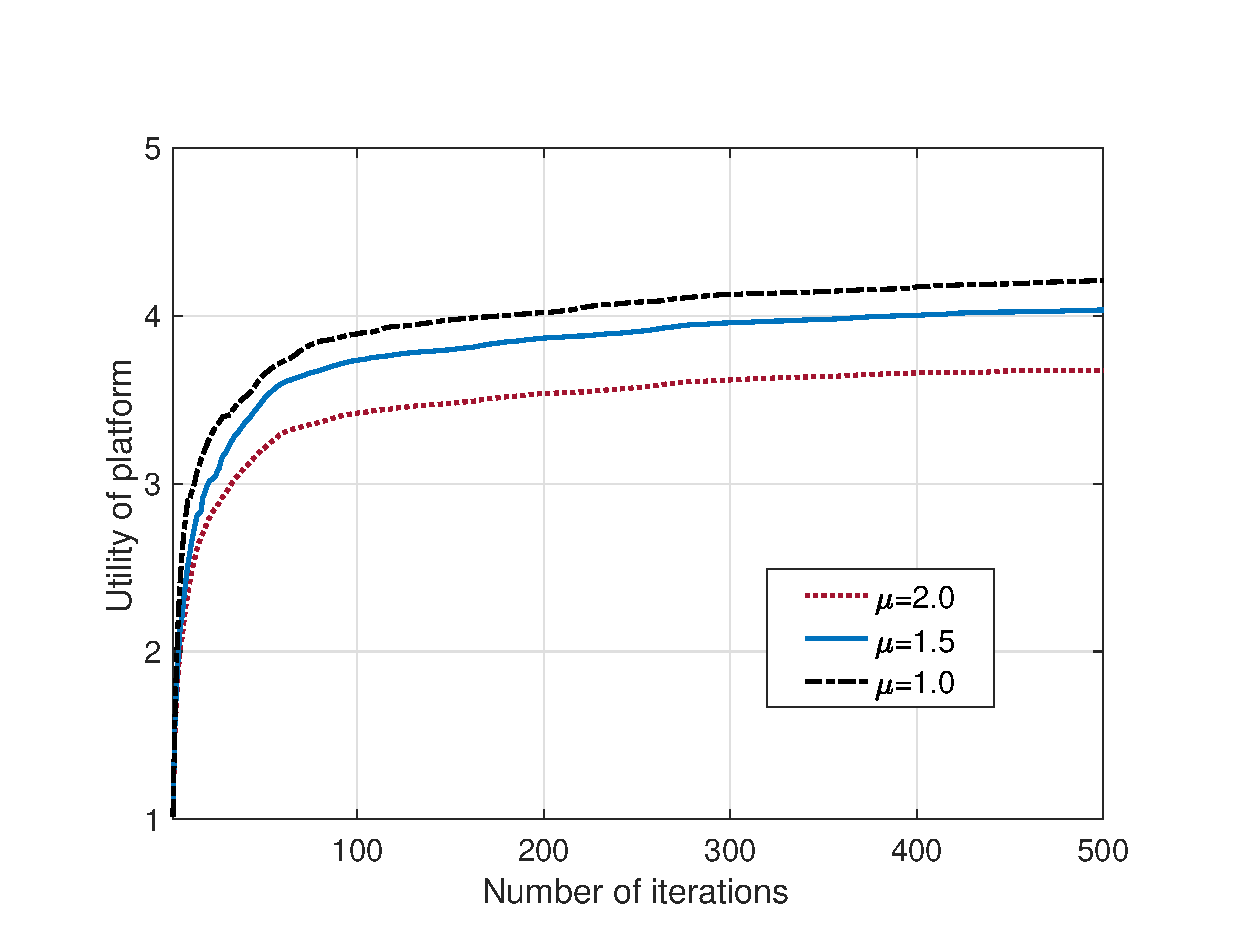
\includegraphics[scale=0.44]{./pic/conv4.eps}
\caption{Illustration of the convergence performance of the learning algorithm.}\label{conv}
\end{figure}
\begin{figure}[t]
%\hspace{-0.35cm}
\centering
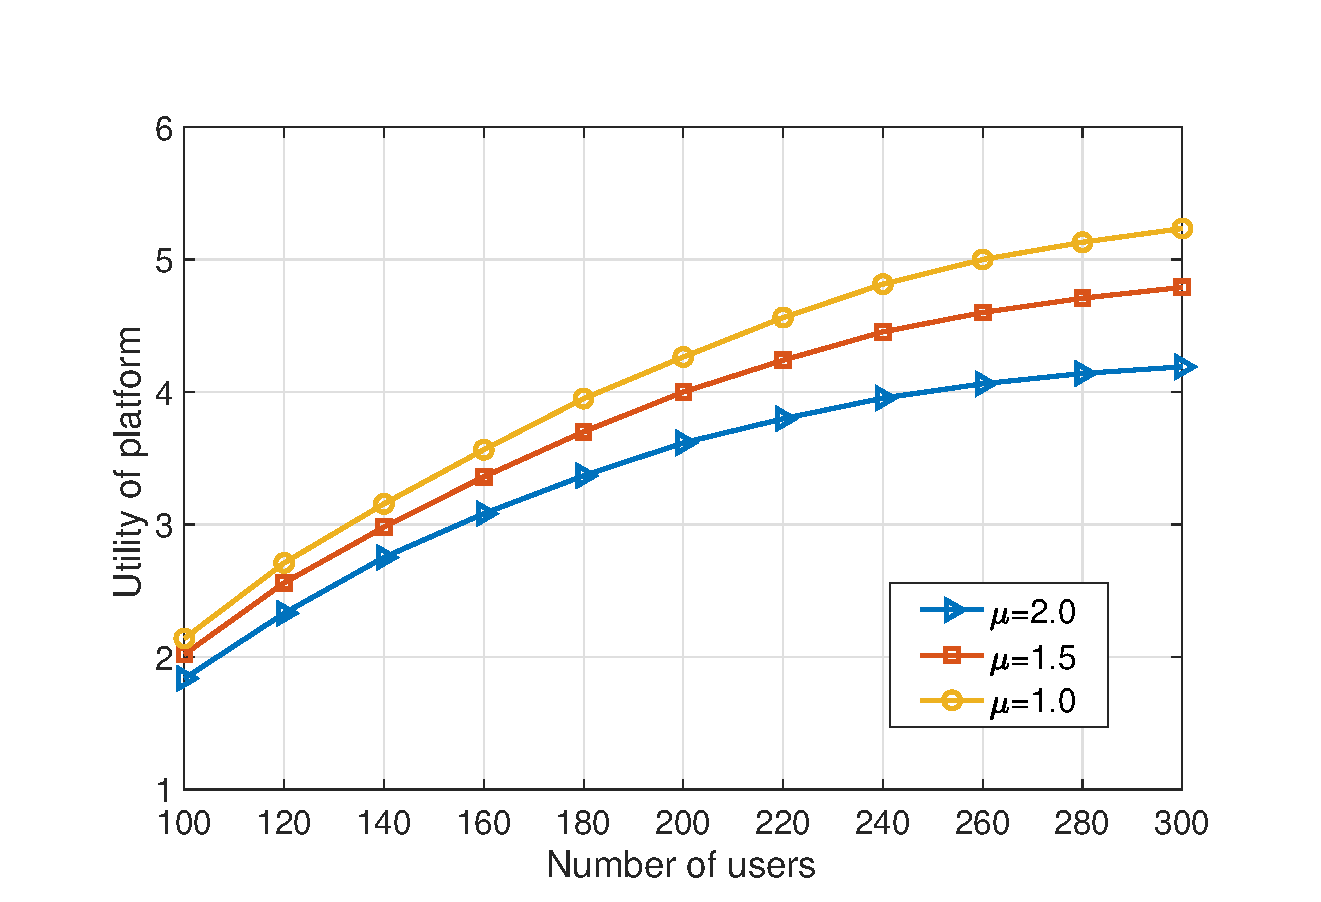
\includegraphics[scale=0.44]{./pic/u_num4.eps}
\caption{Illustration of the impact of amount of users on the platform utility.}\label{cmax}
\end{figure}


\section{Conclusion}\label{sec:s5}
In this article, we give an overview of several state-of-art privacy-preserving approaches for mobile crowdsensing that stimulate the participation of mobile users with privacy concerns of releasing their sensitive data. To address the challenge that participated users' privacy-preserving requirements may be time-varying, we proposed a Q-learning based pricing mechanism through which the MCS platform can dynamically adapt its pricing policy to optimize its utility. A case study is further provided to evaluate the performance of our proposed approach.

